\documentclass[border=10pt]{standalone}
\usepackage{tikz}
\usetikzlibrary{arrows.meta}

\begin{document}
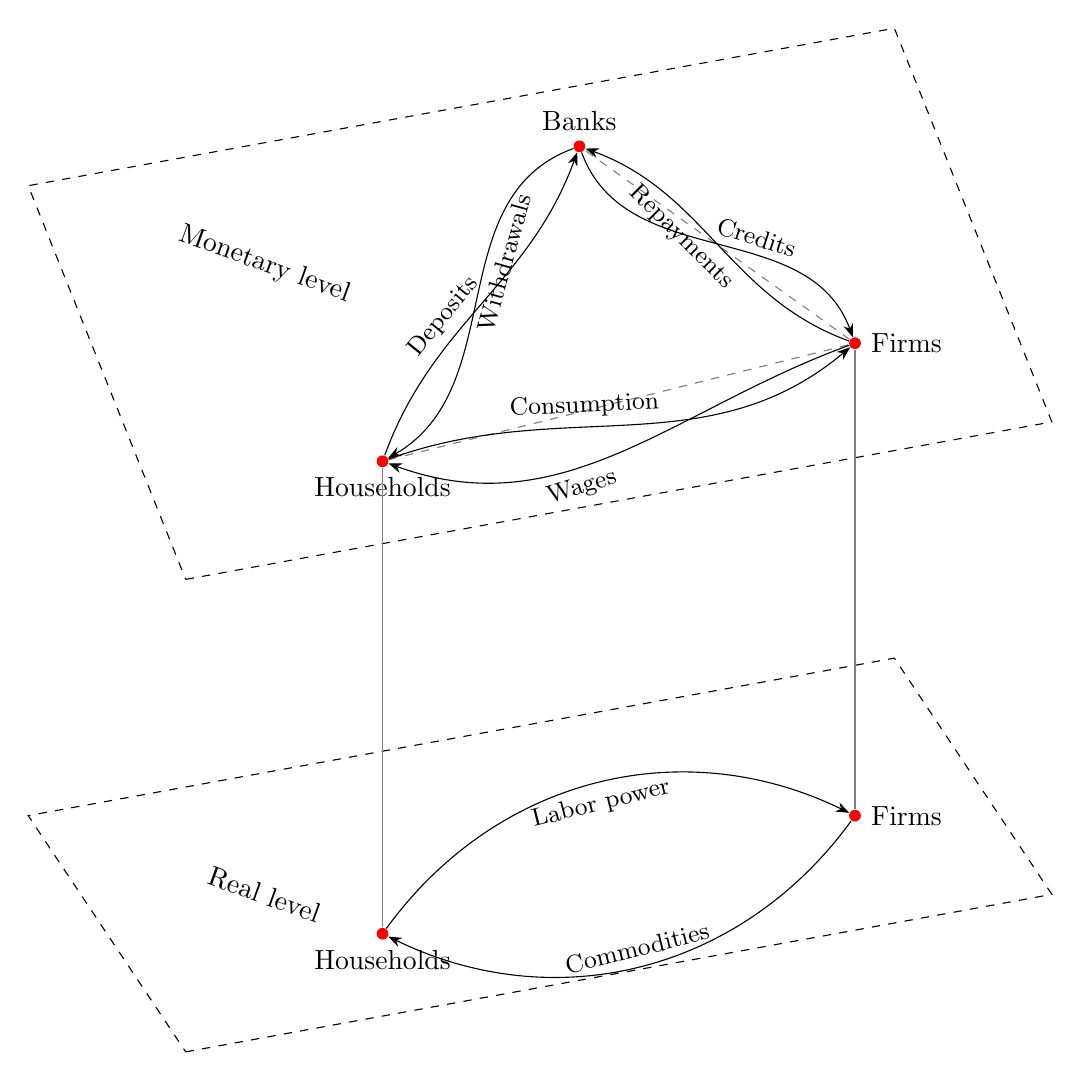
\begin{tikzpicture}[
    >=Stealth,
    node_style/.style={circle, fill=red, inner sep=1.5pt},
    flow_label_style/.style={sloped, midway, font=\small}
]

% Define coordinates for nodes
\node[node_style, label=above:Banks] (mb) at (2.5, 4) {};
\node[node_style, label=right:Firms] (mf) at (6, 1.5) {};
\node[node_style, label=below:Households] (mh) at (0, 0) {};

\node[node_style, label=right:Firms] (rf) at (6, -4.5) {};
\node[node_style, label=below:Households] (rh) at (0, -6) {};

% Draw planes
\draw[dashed] (-2.5, -1.5) -- (8.5, 0.5) -- (6.5, 5.5) -- (-4.5, 3.5) -- cycle;
\node at (-1.5, 2.5) [rotate=-20] {Monetary level};

\draw[dashed] (-2.5, -7.5) -- (8.5, -5.5) -- (6.5, -2.5) -- (-4.5, -4.5) -- cycle;
\node at (-1.5, -5.5) [rotate=-20] {Real level};

% Draw faint triangle connecting monetary nodes
\draw[gray, thin, dashed] (mh) -- (mf) -- (mb) -- cycle;

% Draw inter-level connectors
\draw[gray, thin] (mh) -- (rh);
\draw[gray, thin] (mf) -- (rf);

% Draw flows in a specific order to handle crossings correctly
% Monetary flows (from bottom-most to top-most)
\draw[->] (mf) to[out=160, in=-20] node[flow_label_style, below, pos=0.6] {Repayments} (mb);
\draw[->] (mb) to[out=-160, in=30] node[flow_label_style, below, pos=0.4] {Withdrawals} (mh);
\draw[->] (mh) to[out=70, in=-110] node[flow_label_style, above, pos=0.4] {Deposits} (mb);
\draw[->] (mf) to[out=200, in=-20] node[flow_label_style, below, pos=0.6] {Wages} (mh);
\draw[->] (mh) to[out=20, in=220] node[flow_label_style, above, pos=0.4] {Consumption} (mf);
\draw[->] (mb) to[out=-70, in=110] node[flow_label_style, above, pos=0.6] {Credits} (mf);

% Real flows
\draw[->] (rh) to[bend left=40] node[flow_label_style, below] {Labor power} (rf);
\draw[->] (rf) to[bend left=40] node[flow_label_style, above] {Commodities} (rh);

\end{tikzpicture}
\end{document}